\documentclass[11pt,a4paper]{article}
\usepackage[utf8]{inputenc}
\linespread{2.0}
\renewcommand{\rmdefault}{phv} % Arial
\renewcommand{\sfdefault}{phv} % Arial
\usepackage{geometry}
\usepackage{tabu}
\usepackage{natbib}
\usepackage{amsmath}
\usepackage{graphicx}
\bibliographystyle{abbrvnat}
\setcitestyle{authoryear,open={(},close={)}}
\geometry{a4paper,left=2cm,right=2cm,top=2cm,bottom=2cm}
\font\myfont=cmr12 at 30pt
\title{\myfont Symbolic Regression in Modelling Population Growth}
\author{Wang YuHeng }
\date{December 2018}
\usepackage{natbib}
\usepackage{graphicx}
\begin{document}
\maketitle
\begin{center}
\vspace{8.8cm}
Affliation: Faculty of Natural Sciences, Department of Life Sciences (Silwood Park)
\\
Email: yuheng.wang18@imperial.ac.uk
\\
Words in text: 1876
\end{center}
\newpage

\section{Key words}
Reverse-engineering; Symbolic regression; Population growth; Logistic equation; Lotka–Volterra model 



\section{Introduction}
There are two main different types of models in biological area: mechanistic and phenomenological models. Mechanistic models focus on explaining the mechanisms under the certain pattern or process by extracting mathematical structure from existing theoretical basis. While phenomenological models are just used to fit empirical data with no assumption made. The challenge of developing a mechanistic model is that doing so requires background knowledge about import interactions behind governing the system and their functional forms which are usually beyond the reach \citep{BenjaminT.MartinStephanB.Munch2018}. Another shortage of mechanistic model is that the inherent complexity of biological systems gives rise to complicated mechanistic models with a large number of parameters \citep{Transtrum2016}, making it hard to solve and time consuming. Under some circumstances, building a phenomenological model seems to be more realistic but it is also hard to find correct mathematical structure from empirical data. Reverse engineering like symbolic regression can be used to solve these problems since it can form a variety of function and choose from function set automatically \citep{BenjaminT.MartinStephanB.Munch2018}. Another advantage of symbolic regression is that it can demonstrate mathematical function intuitively. Contrast to other machine learning methods like random forest or neural network, it provides ecologists with opportunity to explore inner mechanisms by giving them certain mathematical structure.

The symbolic regression is barely used in processing biological data \citep{Liu2016}. Inspired by some researchers using symbolic regression in describing physical system \citep{Schmidt2009}. \citet{BenjaminT.MartinStephanB.Munch2018} proposed applying symbolic regression to several classic demographic datasets including self-regulation, predation and cannibalism. A typical function describing population growth is called logistic equation, formalized by differential equation:
\begin{equation}
\frac{dP}{dt} = rP \cdot (1- \frac{P}{K})
\end{equation}
where r means growth rate and K means carrying capacity \citep{mckendrick_pai_1912}.

And this mini-project aims on reproducing symbolic regression on self-regulation population growth. We will test whether symbolic regression performs well in population growth dataset, and try to reproduce the results of \citet{BenjaminT.MartinStephanB.Munch2018}. We find that: (1) symbolic regression has ability of fitting population dataset and reaching equations whose structure is similar to logistic equation, (2) our equation does not explain the variance as good as \citet{BenjaminT.MartinStephanB.Munch2018}, our final coefficient of determination was 0.81 while they got 0.95, the reason causing this will be discussed in this paper.

\section{Methods}
\subsection{Principle of symbolic regression}
Symbolic regression is a machine learning algorithm that aims to identify the mathematical expression that best describe a relationship. At the beginning, a population of random formulas are built to represent a relationship between independent variables and dependent variables. The random expressions are formalised as S-expression \citep{Mccaatity}, consisting several blocks including variables, constant and mathematical operators. It also can be represented as a syntax tree (Figure 1). 
\begin{figure}[h!]
\centering
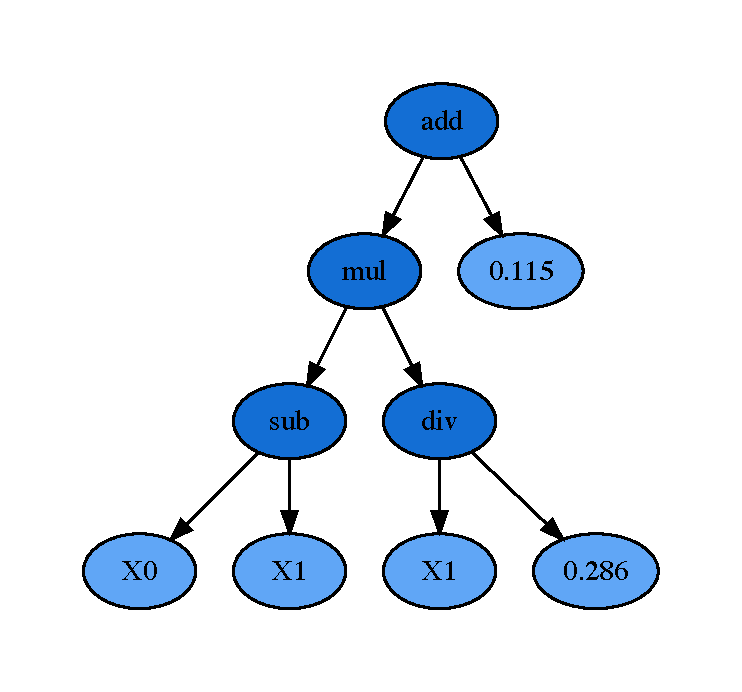
\includegraphics[scale = 0.6]{../Results/Syntax_tree.pdf}
\caption{Expression represented as a syntax tree. This is the tree we got to best describe self-regulation population growth, which is a Lotka – Volterra like equation.}
\end{figure}

After first generation, each expression within population is tested and selected using tournament selection \citep{Brad1995} to create next generation. During this stage, genetic operation including crossover, reproduction, hoist mutation, sub-tree mutation and point mutation are done to the fittest individuals, creating next generation. When doing crossover, the algorithm operates tournament selection twice to find parents expression, and each parent donates one part to generate new individual. Sub-tree mutation is similar to crossover, only more aggressive, because one of the parents is generated randomly instead of tournament selection. Reproduction simply means copy individual to next generation while point mutation means substitute some of winner equation's nodes randomly. Hoist mutation 'prunes' winner syntax tree randomly to make next generation, which mitigates over fitting and decreases model complexity to some degree. Parsimony coefficient is also used to decline model length by giving penalty to more complicated model in the progress of selection. After certain generations, or when lose, residual mean squared error (RMSE) in this case, is less than giving value, the algorithm will output fittest individual in the last generation. 

\subsection{Implementing symbolic regression}
We used the most popular symbolic regression package in python named 'gplearn' in this study. Firstly, we used min max normalization to bring all values into the range [0,1] for several reasons: (1) This operation would eliminate the impact of the unit, making all of the variables in the same dimension and the same scale, therefore,
characteristics of different dimensions can be compared, which greatly improves the accuracy of the regression, (2) normalising data could also speed up the algorithm, (3) 'gplearn' need us to set the constant range in order to find target more quickly, and data normalization will make this step easier. Then, we used following parameters to implement the symbolic regression. The initial population size was 6000, and the number of generation was 25. The initial tree depths for the initial population was chosen from 3 to 6, and the initial method to build first population was 'half and half', which means half of trees‘ function were chosen until initial depths were reached while another half of trees’ function were chosen randomly, allowing trees smaller than initial depth allows. This method provided the population with maximum diversity. The constants range was from -1 to 1, and the parsimony coefficient was chosen as 0.005. Each generation, twenty random individuals were chosen using tournament selection, the fittest individual in this subset was then selected to move on to the next generation. The next generation was constructed through crossover (0.7), sub-tree mutation (0.08), point mutation (0.1), hoist mutation (0.07) and reproduction (0.05). Model fitness were calculated using mean squared error of residuals with in-sample data and out-of-bag data. This was achieved by using bootstrap \citep{Efron} to ensure that the results were robust. Each round, 95\% of data were chosen as in-sample data and 5\% of data were out-of-bag data. 
\begin{figure}[h!]
\centering
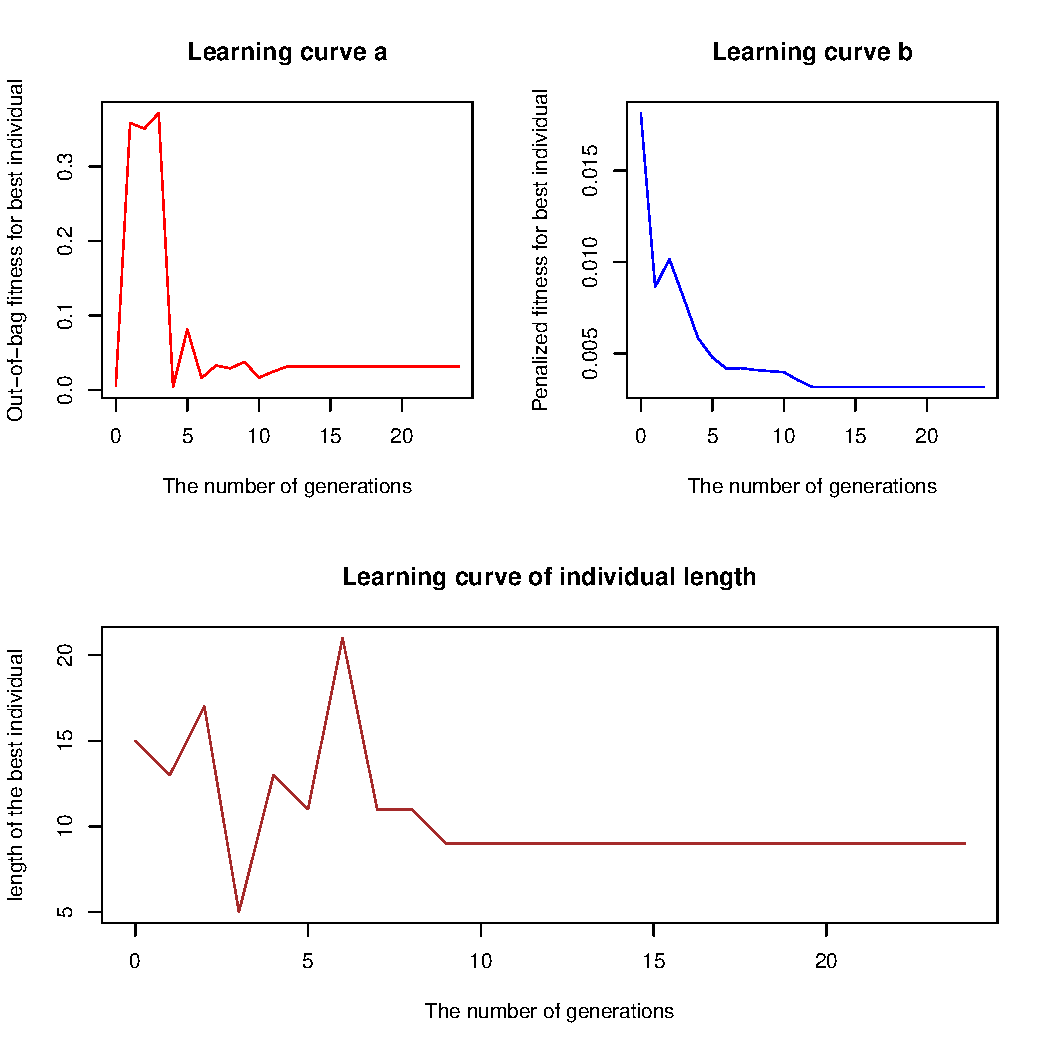
\includegraphics[scale = 0.6]{../Results/log_of_regression.pdf}
\caption{Learning curve of Out-of-bag fitness, penalized fitness and individual expression length for 25 generations. Points in the line represent the best individual within a generation. They all converged after about 15 generations.}
\end{figure}
(Figure 2) shows the learning curve of symbolic regression. We can see that penalized fitness, out-of-bag fitness along with individual length tended to converge after 15 generation, which means fifteen generations were enough for this problem. We can see that the out-of-bag fitness have some outlier values at the beginning, probably because out-of-bag samples were not enough to maintain robust. It is normal to have some intense fluctuation in individual length at the beginning of regression because all generations were generated from random process. 

We divided the raw data into training set and test set. We built the model from training set and calculated the coefficient of determination ($R^{2}$) with test set. About model selection criteria, symbolic regression try to find Pareto front—the set of models that have the best goodness-of-fit for each level of model complexity instead of using Akaike information criterion (AIC) or Bayesian information criterion (BIC) \citep{BenjaminT.MartinStephanB.Munch2018}. We also applied another two non-liner regression algorithm: random forest \citep{Ho1995} and decision tree \citep{Kami2018} on the same dataset, comparing them with the symbolic regression algorithm.

\subsection{Computing languages}
R in version 3.51, Python in version 3.56, and bash were used in this project. We used Python to do symbolic regression, decision tree, random forest and some other kinds of data processing like normalization because Python has many handy package. We can build our program with existing machine learning framework, avoiding lots of repetitive work. We used R to manage the result data and draw the plot because it is really easy to do data management and visualization with some packages in R. Bash script was used to count the words of latex file and patch together the computing workflow.

\section{Data}
We used Paramecium population growth dataset, which comes from the data of \citet{BenjaminT.MartinStephanB.Munch2018}. It consists of four variables: record time, Paramecium population density, nutrient concentration and differential of Paramecium population density versus time, each variable has 56 observations. Paramecium population density and nutrient concentration were used as independent variables to predict differential of Paramecium population density versus time, forming differential equation of population growth.

\section{Results}
From symbolic regression, we got the S-expression:
\begin{figure}[h!]
\centering
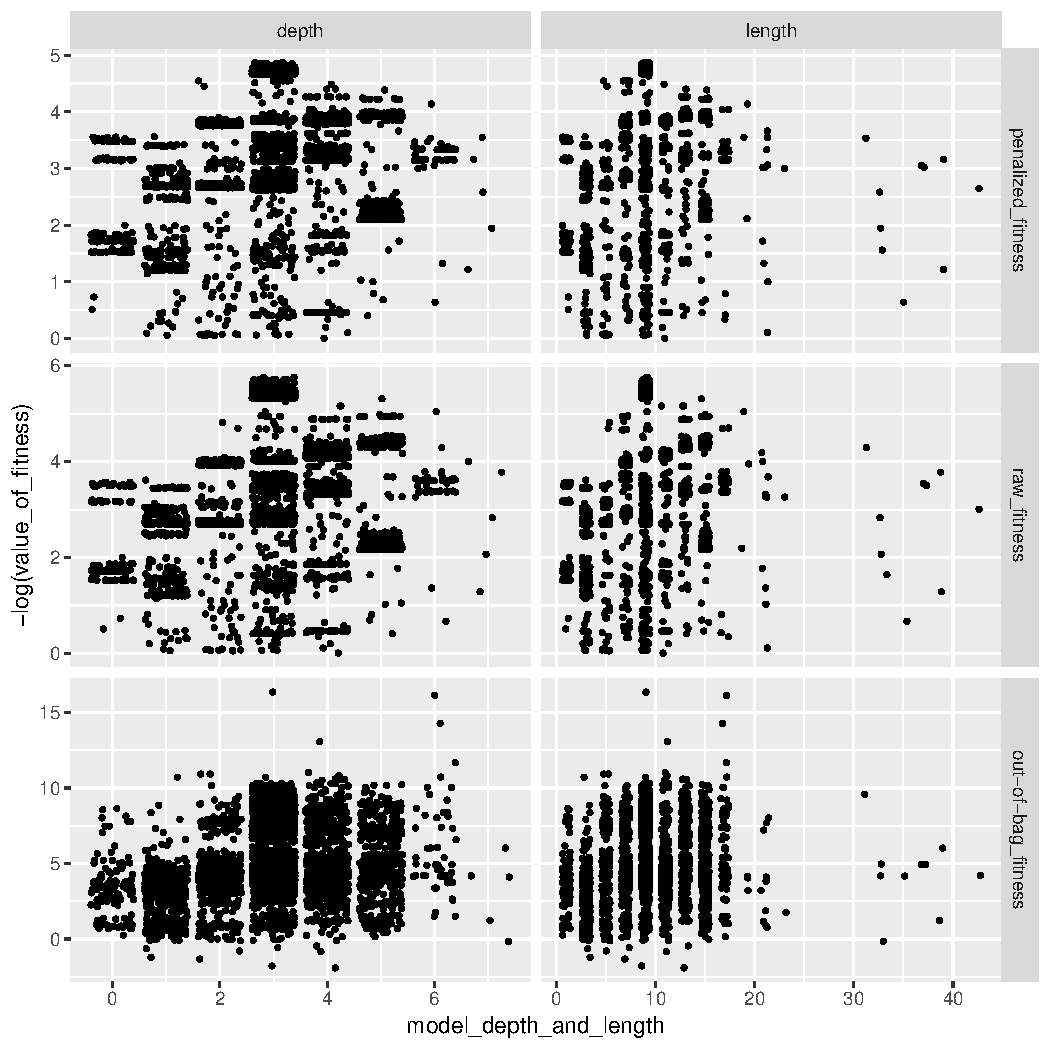
\includegraphics[scale = 0.6]{../Results/model_fitness.pdf}
\caption{The plot shows different types of fitness based on model length and model depth on all of the last generation's models. Depth means the maximum depth of the program tree. Length means the number of functions and terminals in the program. The value of fitness are RMSE, processed with -log for better visualization. Plots are jittered in the horizontal direction for visualization. Plots on the first row show penalized fitness for different models, while raw fitness are shown on the second row and out-of-bag fitness are shown on the third row. }
\end{figure}
add(mul(sub(x0,x1),div(x1,0.286)),0.115), translating it into standard differential equation:
\begin{equation}
    \frac{dP}{dt} = 3.5N \cdot P \cdot (1- \frac{P}{N}) + 0.115
\end{equation}
where N means nutrient concentration and P means Paramecium population density, stating that Paramecium dynamics is governed by nutrient concentration and Paramecium population density. We can easily find that this is exactly the form of Lotka–Volterra model, 3.5N represents growth rate and N represents carrying capacity. The only difference is that this model adds a constant at the end of the equation. This result demonstrates that symbolic regression has ability of building a model which represents biological plausible hypothesis. We also drew a plot about different types of fitness versus model length and depth on the last generation (Figure 3).  The best value for penalized fitness, raw fitness and out-of-bag fitness are 7.66e-3, 3.16e-3, 7.854949e-08 respectively. 
\begin{figure}[h!]
\centering
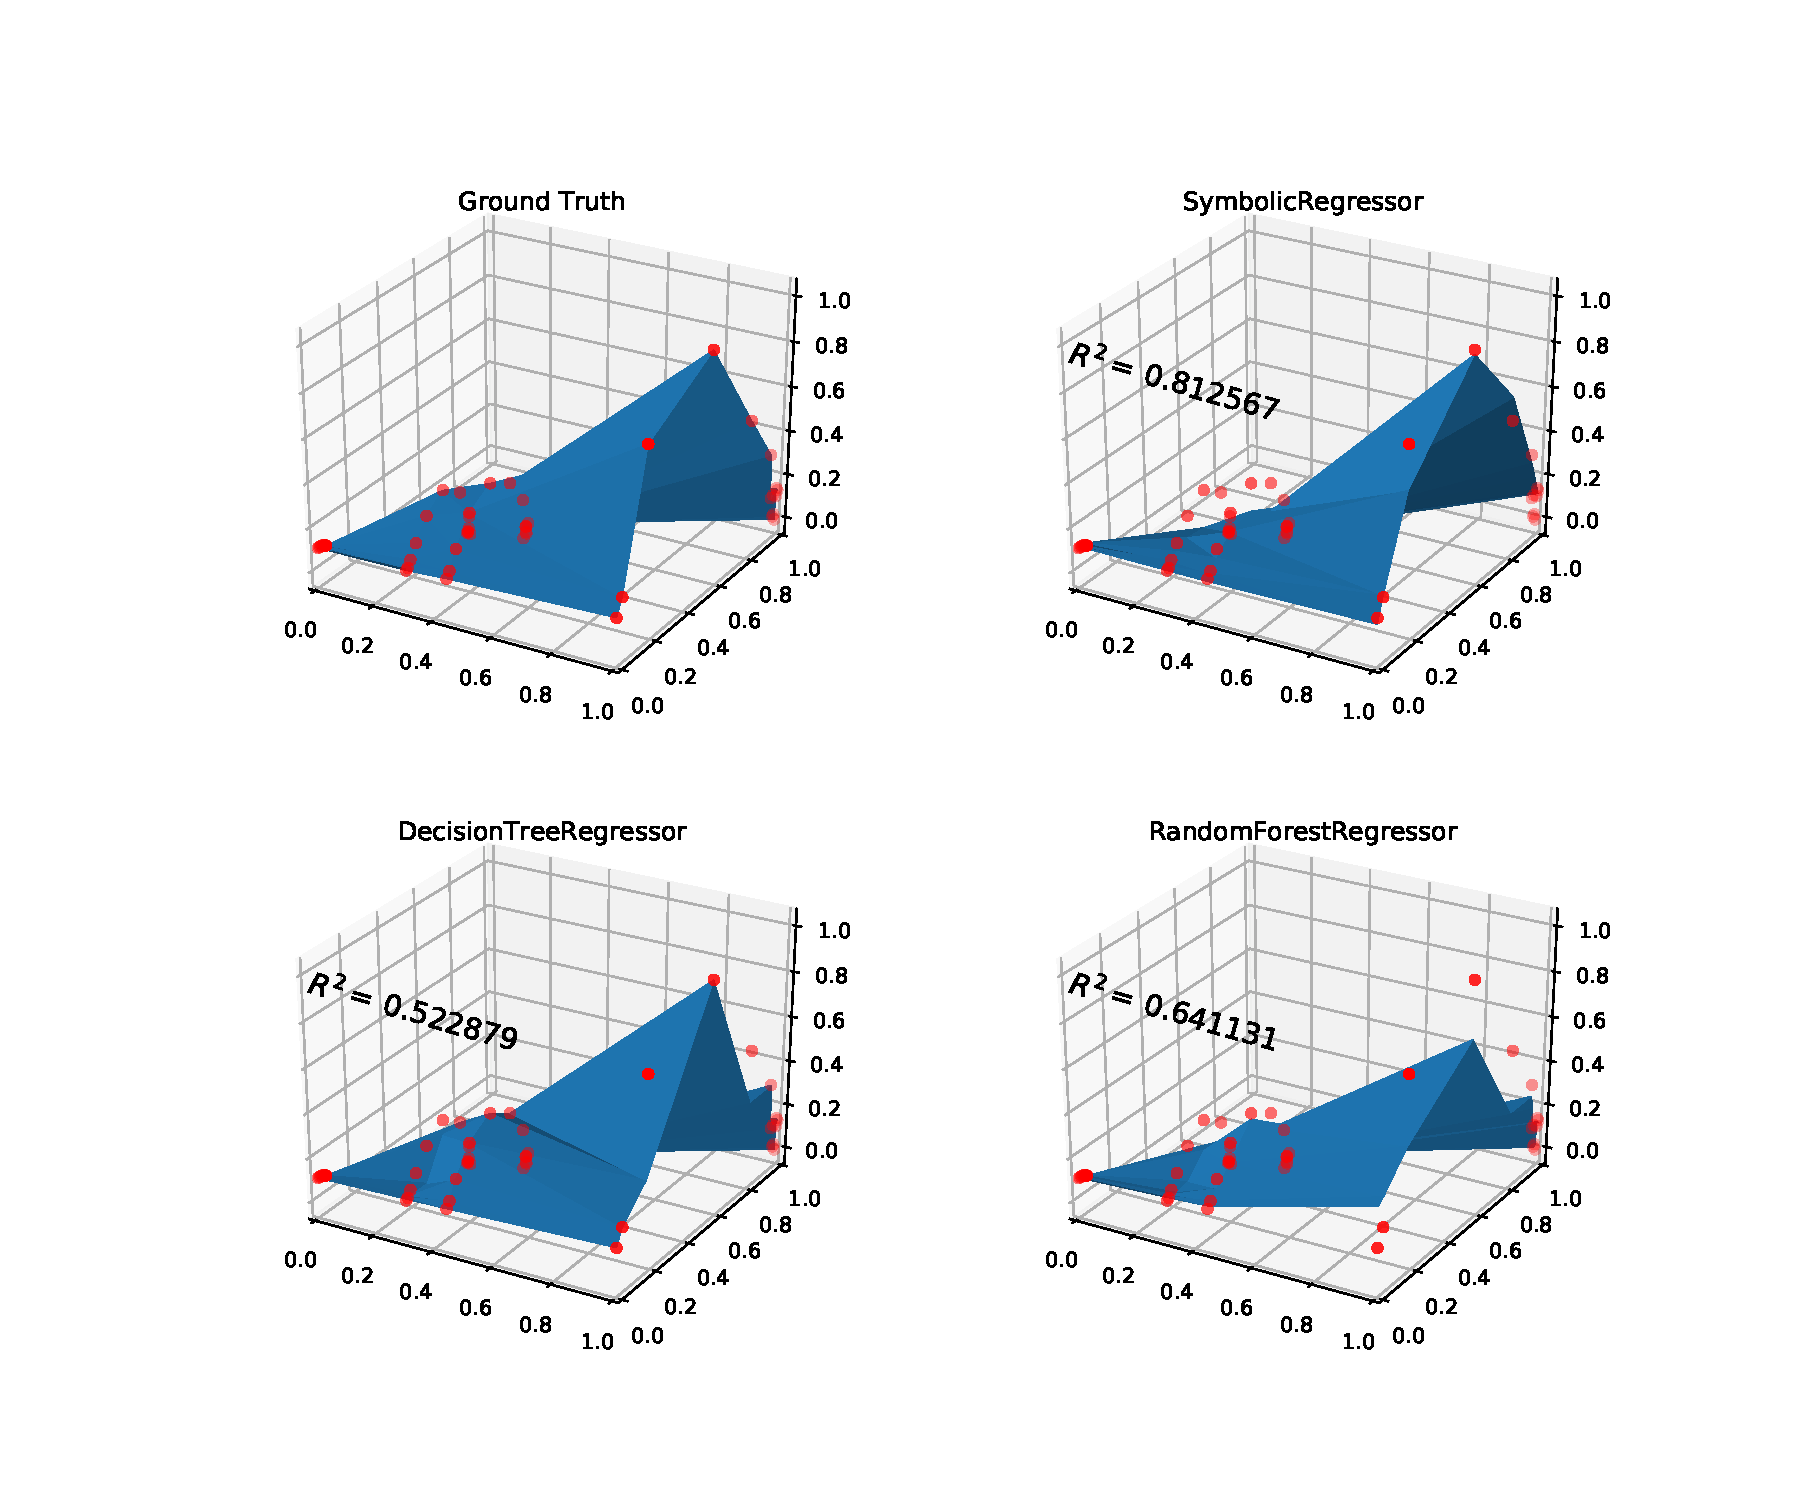
\includegraphics[scale = 0.52]{../Results/gp_vs_rf_dt.pdf}
\caption{The plot shows the model fitting accuracy of symbolic regression, decision tree and random forest. The blue surface is the prediction from different algorithms and red points are dependent variables ($\frac{dP}{dt}$) of ground truth.}
\end{figure}
They are all found in depth 3 and length 9 models, which share the same structure with Lotka–Volterra model. Most models are concentrated in length from 1 to 20 and depth from 0 to 6. Model fitness grow as the model length and depth increase at first, after peaking at length 9 and depth 3, the fitness begin to decrease. The result is slightly different from \citeauthor{BenjaminT.MartinStephanB.Munch2018}'s paper where the model fitness should increase and maintain high as the length and depth of model grow. This may be due to the models within same generation tend to be homogeneous and the number of long models is relatively small. Another reason for this difference is that we did not do constant compression \citep{BenjaminT.MartinStephanB.Munch2018} on this project, resulting that some models are 
artificially long because some unidentifiable parameters exist.  
We also calculated the coefficient of determination of symbolic regression on the test set, comparing with decision tree and random forest (Figure 4). From this plot we can conclude that the symbolic regression is more accurate than other two algorithms in some way because it has the best value of $R^{2}$. But we can not say symbolic regression is better arbitrarily as parameters on decision tree and random forest were far from perfect. What we can say is that symbolic regression has an excellent fitting ability among non-linear regression algorithm.

\section{Discussion}
By generating lots of model and operating evolution, symbolic regression find the model most explaining the variance in data. The model generated and selected by symbolic regression shares the same structure with classical ecological model. This can not be guaranteed but encourages us that the possibility that ecological plausible hypothesis are contained in symbolic regression's model set is pretty large. Since that, we may apply symbolic regression on other biological process like thermal performance curves (TPCs) \citep{Luhring2017}. Since TPCs question has many hypothesis, symbolic regression can compare them with each other as well as thousands of alternative models. Or we can apply symbolic regression on some unknown biological process to help us explore the potential mechanisms since symbolic regression output the explicit equation. At the same time, we have to be careful to use symbolic regression to avoid over fitting and to make sure the result models are robust. This could be done by several machine learning techniques like cross validation and bootstrap. 

Our result did not reach the $R^{2}$ value as good as \citet{BenjaminT.MartinStephanB.Munch2018}, mainly because they separated the process of equation building and parameter estimation. They firstly used symbolic regression to generate the model and then used restricted back-propagation \citep{Riedmiller92rprop-} to estimate parameter values, while the package we used combines these two steps together by generating value of parameters directly from symbolic regression. As a consequence, our algorithm has more complexity and less accuracy than theirs. We have to admit that original author's program is better although 'gplearn' is the most popular symbolic regression package in python. 

\newpage
\bibliographystyle{plain}
\bibliography{references}
\newpage

\end{document}
